% !TeX program = pdflatex
\documentclass[tikz,border=8pt]{standalone}
\usepackage{tikz}
\usetikzlibrary{calc}
\definecolor{FigureBlue}{HTML}{2563EB}
\definecolor{FigureOrange}{HTML}{EA580C}
\definecolor{FigureSlate}{HTML}{64748B}
\begin{document}
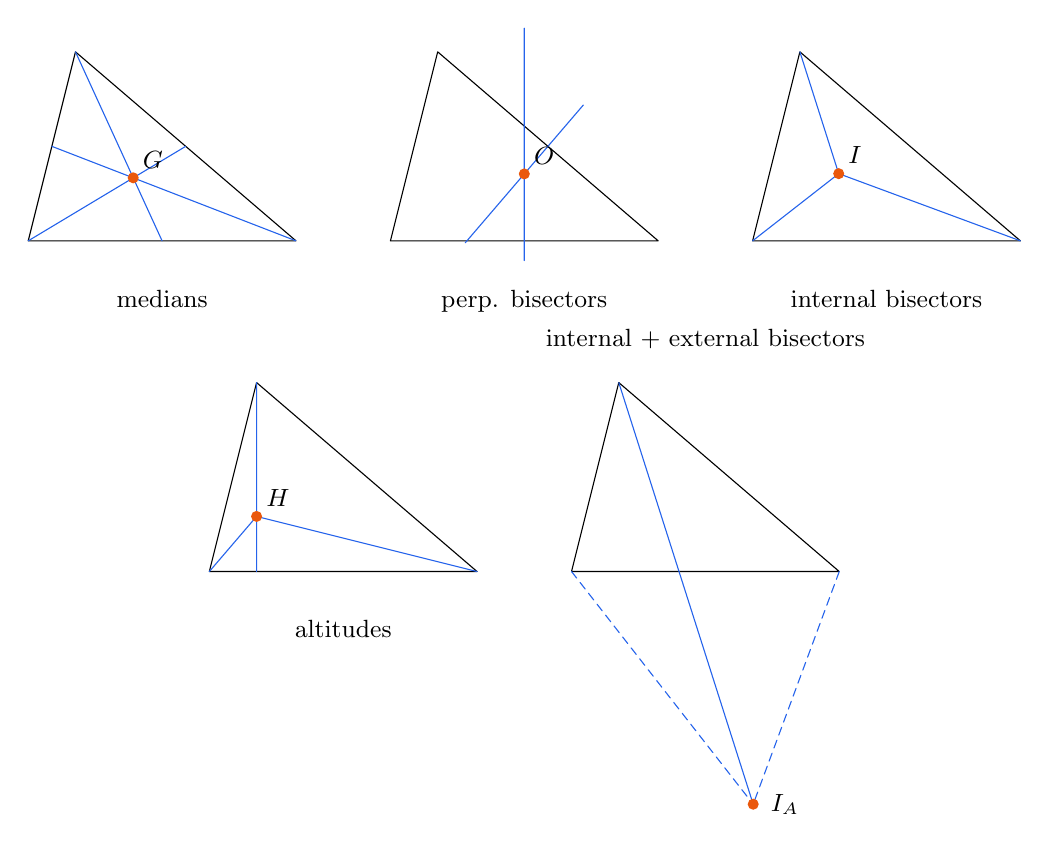
\begin{tikzpicture}[line cap=round,line join=round,font=\small]
  \begin{scope}
    \coordinate (A) at (.6,2.4);\coordinate (B) at (0,0);\coordinate (C) at (3.4,0);
    \coordinate (Ma) at ($(B)!.5!(C)$);\coordinate (Mb) at ($(C)!.5!(A)$);\coordinate (Mc) at ($(A)!.5!(B)$);
    \coordinate (G) at (1.3333,.8);
    \draw (A)--(B)--(C)--cycle;\draw[FigureBlue] (A)--(Ma) (B)--(Mb) (C)--(Mc);
    \fill[FigureOrange] (G) circle (2pt);\node[above right] at (G) {$G$};\node[below=5mm] at (Ma) {medians};
  \end{scope}
  \begin{scope}[xshift=4.6cm]
    \coordinate (A) at (.6,2.4);\coordinate (B) at (0,0);\coordinate (C) at (3.4,0);\coordinate (O) at (1.7,.85);
    \draw (A)--(B)--(C)--cycle;\draw[FigureBlue] (1.7,-.25)--(1.7,2.7) (.95,-.025)--(2.45,1.725);
    \fill[FigureOrange] (O) circle (2pt);\node[above right] at (O) {$O$};\node[below=5mm] at (1.7,0) {perp. bisectors};
  \end{scope}
  \begin{scope}[xshift=9.2cm]
    \coordinate (A) at (.6,2.4);\coordinate (B) at (0,0);\coordinate (C) at (3.4,0);\coordinate (I) at (1.093,.853);
    \draw (A)--(B)--(C)--cycle;\draw[FigureBlue] (A)--(I) (B)--(I) (C)--(I);
    \fill[FigureOrange] (I) circle (2pt);\node[above right] at (I) {$I$};\node[below=5mm] at (1.7,0) {internal bisectors};
  \end{scope}
  \begin{scope}[yshift=-4.2cm,xshift=2.3cm]
    \coordinate (A) at (.6,2.4);\coordinate (B) at (0,0);\coordinate (C) at (3.4,0);\coordinate (H) at (.6,.7);
    \draw (A)--(B)--(C)--cycle;\draw[FigureBlue] (A)--(.6,0) (B)--(H) (C)--(H);
    \fill[FigureOrange] (H) circle (2pt);\node[above right] at (H) {$H$};\node[below=5mm] at (1.7,0) {altitudes};
  \end{scope}
  \begin{scope}[yshift=-4.2cm,xshift=6.9cm]
    \coordinate (A) at (.6,2.4);\coordinate (B) at (0,0);\coordinate (C) at (3.4,0);\coordinate (Ia) at (2.307,-2.955);
    \draw (A)--(B)--(C)--cycle;\draw[FigureBlue] (A)--(Ia);
    \draw[FigureBlue,densely dashed] (B)--(Ia) (C)--(Ia);
    \fill[FigureOrange] (Ia) circle (2pt);\node[right=1mm] at (Ia) {$I_A$};
    \node[above=3mm] at (1.7,2.4) {internal + external bisectors};
  \end{scope}
\end{tikzpicture}
\end{document}
